\documentclass[10pt]{article}

\usepackage[T1]{fontenc}
\usepackage[utf8]{inputenc}
\usepackage{lmodern}
\usepackage{amsmath,amssymb,amsthm}
\usepackage{mathtools}
\usepackage{booktabs}
\usepackage{float}
\usepackage{microtype}
\usepackage{tikz}
\usetikzlibrary{calc}
\usepackage[margin=1in]{geometry}
\usepackage[hidelinks,hyperfootnotes=false]{hyperref}
\urlstyle{same}

\title{The Circle Problem of Gauss and the Divisor Problem of Dirichlet---Still Unsolved}
\author{Bruce C. Berndt, Sun Kim, and Alexandru Zaharescu}
\date{}

\newcommand{\floor}[1]{\left\lfloor #1\right\rfloor}
\newcommand{\sump}{\sideset{}{'}\sum}

\theoremstyle{plain}
\newtheorem{theorem}{Theorem}
\newtheorem{entry}[theorem]{Entry}
\newtheorem{corollary}[theorem]{Corollary}

\begin{document}
\maketitle


\begin{abstract}
Let $r_{2}(n)$ denote the number of representations of the positive integer $n$ as a sum of two squares, and let $d(n)$ denote the number of positive divisors of $n$. Gauss and Dirichlet were evidently the first mathematicians to derive asymptotic formulas for $\sum_{n \leq x} r_{2}(n)$ and $\sum_{n \leq x} d(n)$, respectively, as $x$ tends to infinity. But what is the error made in such approximations? Number theorists have been attempting to answer these two questions for over one and one-half centuries, and although we think that we essentially ``know'' what these errors are, progress in proving these conjectures has been agonizingly slow. Ramanujan had a keen interest in these problems, and although, to the best of our knowledge, he did not establish any bounds for the error terms, he did give us identities that have been used to derive bounds, and two further identities that might be useful, if we can figure out how to use them. In this paper, we survey what is known about these two famous unsolved problems, with a moderate emphasis on Ramanujan's contributions.
\end{abstract}

\section{Introduction}

If $a(n)$ is an arithmetical function, i.e., a function defined on the positive integers, number theorists frequently want to know how large (or small) it is and what its average size is. It is the latter question, focusing on two famous arithmetical functions, that we address in this survey. Usually, however, number theorists are not satisfied with knowing only the ``average'' of $a(n)$; they also want to ascertain the error made in their determination of this ``average.'' To be more precise, the average order of $a(n)$ is defined by

$$
\frac{1}{x} A(x):=\frac{1}{x} \sum_{n \leq x} a(n),
$$

and we first want to determine a function $M(x)$ such that

$$
\lim _{x \to \infty} \frac{A(x)}{M(x)}=1 .
$$

But we want to know more. If we write


\begin{equation*}
A(x)=M(x)+E(x), \tag{1.1}
\end{equation*}


what is the size or order of the ``error term'' $E(x)$ as $x \to \infty$? The most useful attacks on such problems employ analysis. Since $A(x)$ is discontinuous, it might be difficult to use continuous or analytic functions in such an approach. Sometimes it may be more advantageous to consider a weighted average, e.g.,

$$
A_{q}(x):=\sum_{n \leq x} a(n)(x-n)^{q}, \quad q>0 .
$$

Of course, $A_{q}(x)$ is still discontinuous, but it is ``smoother'' than $A_{0}(x):=A(x)$. What do we mean by ``smoother''? Generally (but admittedly very roughly), arithmetical

\begingroup
\renewcommand{\thefootnote}{}
\footnotetext{\href{https://doi.org/10.1080/00029890.2018.1401853}{doi.org/10.1080/00029890.2018.1401853};
MSC: Primary 11-03, Secondary 11N37; 11P21. Color versions of one or more figures in the original article can be found online at
\href{https://www.tandfonline.com/uamm}{www.tandfonline.com/uamm}.}
\endgroup
functions are often small for small $n$ and large for large $n$. For large $x$, the factor $(x-n)^{q}$ is large for small $n$ and small for large $n$, thus ``evening out'' the terms in the sum. Of course, we must have some means to obtain information about $A(x)$ from $A_{q}(x), q>0$.

The purpose of this paper is to survey what is known about the average order of two of the most important arithmetical functions in number theory, $r_{2}(n)$ and $d(n)$, defined in the abstract and defined in more detail below. We shall see that determining their ``error terms'' constitutes two of the most famous, difficult, unsolved problems in number theory.

\paragraph{Definitions.} The arithmetical function $r_{2}(n)$ denotes the number of representations of the positive integer $n$ as a sum of two squares, where the convention is that different signs and different orders of the summands yield distinct representations. Thus, $r_{2}(13)=8$, because $13=(\pm3)^{2}+(\pm2)^{2}=(\pm2)^{2}+(\pm3)^{2}$. The circle problem (to be described more precisely later) is to determine the average order of $r_{2}(n)$ as well as the order of the error term $E(x)$ in (1.1).

The arithmetical function $d(n)$ equals the number of positive divisors of $n$. Thus, $d(6)=4$ and $d(13)=2$. The Dirichlet divisor problem, or, more briefly, the divisor problem (also to be described more precisely later) is to determine the average order of $d(n)$ as well as the order of the error term $E(x)$.

Although the great Indian mathematician Srinivasa Ramanujan did not leave us any theorems about these error terms, he evidently was passionately interested in these problems and contributed useful identities in attacking these two error terms. Two identities from his lost notebook [33], one connected with $r_{2}(n)$, and the other with $d(n)$, have yet to be employed in the circle and divisor problems. One of these two identities is discussed in detail in Section 6. Perhaps a reader of this survey article will be inspired to find more intimate and useful connections of Ramanujan's identities with these two notoriously difficult, unsolved problems.

We write $f(x)=O(F(x))$, as $x \to \infty$, if there exist positive numbers $C$ and $x_{0}$ such that $|f(x)| \leq C|F(x)|$ whenever $x \geq x_{0}$. We write $f(x)=o(F(x))$, as $x \to \infty$, if $f(x) / F(x) \to 0$ as $x \to \infty$.

Finally, we say that $f(x)=\Omega(F(x))$ as $x \to \infty$ if there exist a sequence $\left\{x_{n}\right\} \to \infty$, $n \geq 1$, and a positive number $C$ such that, for all $n \geq 1,\left|f\left(x_{n}\right)\right|>C\left|F\left(x_{n}\right)\right|$. Similarly, $f(x)=\Omega_{+}(F(x))$ (respectively, $f(x)=\Omega_{-}(F(x))$ ) as $x \to \infty$ if there exist a sequence $\left\{x_{n}\right\} \to \infty$ and a positive number $C$ such that, for all $n \geq 1, f\left(x_{n}\right)>C\left|F\left(x_{n}\right)\right|$ (respectively, $f\left(x_{n}\right)<-C\left|F\left(x_{n}\right)\right|$ ). We write $f(x)=\Omega_{ \pm}(F(x))$, as $x \to \infty$, if both $f(x)=\Omega_{+}(F(x))$ and $f(x)=\Omega_{-}(F(x))$ hold.

\section{The Circle Problem}

Each representation of $n$ as a sum of two squares can be associated with a lattice point in the plane. For example, $13=(-2)^{2}+3^{2}$ can be associated with the lattice point $(-2,3)$. Each lattice point can be associated with a unit square. There are, of course, four possible associated squares, but let us choose that unit square for which the lattice point is in the southwest corner of the square. If we set $r_{2}(0)=1$, then $\sum_{0 \leq n \leq x} r_{2}(n)$ is equal to the number of lattice points lying within a circle of radius $\sqrt{x}$, which is numerically equal to the total area of unit squares whose southwest corners lie within this circle of radius $\sqrt{x}$. The number of lattice points within this circle, or the total of the areas of the associated unit squares, is approximately the area of this circle, $\pi x$. Thus, we can write


\begin{equation*}
R(x):=\sum_{0 \leq n \leq x}^{\prime} r_{2}(n)=\pi x+P(x), \tag{2.1}
\end{equation*}


\begin{figure}[H]
\centering
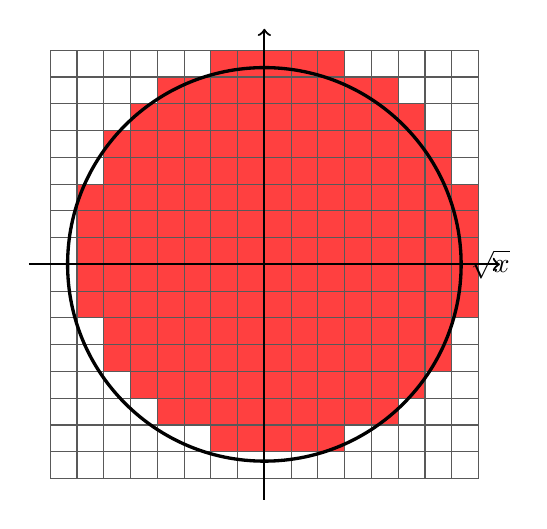
\begin{tikzpicture}[scale=0.34]
  \def\radius{7.35}
  % A unit square is shaded exactly when its southwest corner lies in the disk.
  \foreach \i in {-8,...,7}{
    \foreach \j in {-8,...,7}{
      \pgfmathtruncatemacro{\inside}{(\i*\i+\j*\j <= \radius*\radius) ? 1 : 0}
      \ifnum\inside=1
        \fill[red!75] (\i,\j) rectangle ++(1,1);
      \fi
    }
  }
  \draw[step=1,black!65,thin] (-8,-8) grid (8,8);
  \draw[->,thick] (-8.8,0) -- (8.8,0);
  \draw[->,thick] (0,-8.8) -- (0,8.8);
  \draw[very thick] (0,0) circle[radius=\radius];
  \draw[thick] (0,0) -- (\radius,0);
  \node[right] at (\radius,0) {$\sqrt{x}$};
\end{tikzpicture}
\caption{The circle problem.}
\label{fig:circle-problem}
\end{figure}

where the prime on the summation sign on the left-hand side indicates that if $x$ is an integer, only $\frac{1}{2} r_{2}(x)$ is counted. (It may seem strange that we count only $\frac{1}{2}$ of the lattice points lying on the circle of radius $\sqrt{x}$. It turns out that the sum in (2.1) is the one that naturally arises when we employ analytic techniques, e.g., from Fourier analysis.) Thus, the error made in using the area of the circle of radius $\sqrt{x}$ as our first approximation to the sum on the left-hand side is denoted by $P(x)$. Finding the correct order of magnitude of the error term $P(x)$ as $x \to \infty$ is the circle problem. To the best of our knowledge, in about 1800, C. F. Gauss was the first mathematician to think about the circle problem [12, p. 277], [32, p. 100].

\begin{theorem}
As $x \to \infty$,

\[
P(x)=O(\sqrt{x}).
\]
\end{theorem}

\begin{proof}
From simple geometrical considerations in Figure~\ref{fig:circle-problem}, Gauss observed that

$$
\begin{aligned}
& R(x)<\pi(\sqrt{x}+\sqrt{2})^{2}, \\
& R(x)>\pi(\sqrt{x}-\sqrt{2})^{2} .
\end{aligned}
$$

From these two inequalities, we conclude that

$$
R(x)=\pi x+O(\sqrt{x}),
$$

as $x \to \infty$.
\end{proof}

No further progress was made until 1906 when W. Sierpiński [34] proved that $P(x)=O\left(x^{1 / 3}\right)$. His work, which contains some elements of the circle method, came two years after that of G. F. Voronoï [39], who proved a corresponding result for the divisor problem; see (3.3). E. Landau [25], [27] simplified Sierpiński's ideas but in doing so obtained the weaker result $P(x)=O\left(x^{1 / 3+\epsilon}\right)$, for every $\epsilon>0$. However, in [26],

Landau, in a considerably more difficult argument than that he used in [25] and [27], provided another proof of Sierpiński's theorem.

To describe further progress on the circle problem, it is necessary to introduce the ordinary Bessel function $J_{\nu}(z)$, which is normally defined by


\begin{equation*}
J_{\nu}(z):=\sum_{n=0}^{\infty} \frac{(-1)^{n}}{n!\Gamma(\nu+n+1)}\left(\frac{z}{2}\right)^{\nu+2n}, \quad 0<|z|<\infty, \quad \nu \in \mathbb{C} . \tag{2.2}
\end{equation*}


Of key importance in attacking the circle problem is its asymptotic formula [40, p. 199]


\begin{equation*}
J_{\nu}(x)=\left(\frac{2}{\pi x}\right)^{1 / 2} \cos \left(x-\frac{1}{2} \nu\pi-\frac{1}{4} \pi\right)+O\left(\frac{1}{x^{3 / 2}}\right), \quad x \to \infty . \tag{2.3}
\end{equation*}


After the work of Sierpiński and Landau, most efforts toward obtaining an upper bound for $P(x)$ have ultimately rested upon the identity


\begin{equation*}
\sum_{0 \leq n \leq x}^{\prime} r_{2}(n)=\pi x+\sum_{n=1}^{\infty} r_{2}(n)\left(\frac{x}{n}\right)^{1 / 2} J_{1}(2 \pi \sqrt{n x}), \tag{2.4}
\end{equation*}


with the use of the asymptotic formula (2.3). More precisely, we substitute (2.3) into (2.4). The contribution of the $O$-term in (2.3) to the series in (2.4) yields an absolutely convergent series, which can be trivially estimated. Observe that the contribution of the trigonometric portion of (2.3) gives a series on the right-hand side of (2.4) that converges conditionally and boundedly but not absolutely. Of course, in view of the discontinuities on the left-hand side of (2.4), it would be impossible to have a series converging uniformly on intervals containing positive integers on the right-hand side. Thus, methods must be developed to study the behavior of such trigonometric series for large $x$, so that improvements on the error term $P(x)$ can be achieved.

Readers might be surprised that Bessel functions arise in the study of the circle problem. Those who have taught or taken a course in partial differential equations recall that Bessel functions arise in many physical problems in which there is circular or cylindrical symmetry. There is clearly circular symmetry with the circle problem, and so it should not now be too surprising that Bessel functions make their appearance.

The identity (2.4) was first published and proved in G. H. Hardy's paper [14], [16, pp. 243-263]. In a footnote, Hardy [16, p. 245] remarks, ``The form of this equation was suggested to me by Mr. S. Ramanujan, to whom I had communicated the analogous formula for $d(1)+d(2)+\cdots+d(n)$, where $d(n)$ is the number of divisors of $n$.'' Thus, it appears that Ramanujan was the first to prove (2.4), although we have no record of his proof. Today, the identity (2.4) is frequently referred to as the ``Hardy identity,'' which unfortunately does not reflect any credit to Ramanujan.

Landau [29, p. 188] proved, for $\rho=1$, that

% The printed article has n=0 in the Bessel series below, although x/n is present.
% The correct lower limit is n=1.
\begin{align*}
& \frac{1}{\Gamma(\rho+1)} \sum_{0 \leq n \leq x} r_{2}(n)(x-n)^{\rho} \\
& \quad=\frac{\pi x^{\rho+1}}{\Gamma(\rho+2)}+\frac{1}{\pi^{\rho}} \sum_{n=1}^{\infty} r_{2}(n)\left(\frac{x}{n}\right)^{(\rho+1)/2} J_{\rho+1}(2 \pi \sqrt{n x}) . \tag{2.5}
\end{align*}


Using (2.5) and (2.3), J. E. Littlewood and A. Walfisz [30] and Landau [29, p. 271] proved that


\begin{equation*}
P(x)=O\left(x^{\frac{37}{112}+\epsilon}\right), \tag{2.6}
\end{equation*}


for each $\epsilon>0$. Note that

$$
\frac{37}{112}<\frac{37}{111}=\frac{1}{3} .
$$

A detailed account of the circle problem can be found in Landau's famous treatise [29, pp. 183-303]. In addition to detailed proofs of (2.4), (2.5) (for $\rho=1$ ), and (2.6), proofs of Sierpiński's theorem and the lower bounds of Hardy described below in Section 5 are also given in easy-to-read detail. Several properties of Bessel functions play prominent roles.

We remark that K. Chandrasekharan and R. Narasimhan [10] proved that the identity (2.5) actually holds for every $\rho>-\frac{1}{2}$.

In the century after the work of Sierpiński and Landau, several improvements on the order of magnitude of the error term $P(x)$ were made, with the first by J. G. van der Corput in 1923 [38]. Because bounds for the error term $P(x)$ invariably lead to similar bounds for the error term in the divisor problem, we next discuss this problem before surveying these improvements.

\section{The Dirichlet Divisor Problem}

The Dirichlet divisor problem, or more briefly, the divisor problem, arises from estimating $\sum_{n \leq x} d(n)$. As we describe in more detail below, equivalently, the problem is to estimate the number of lattice points under or on a certain hyperbola. We first offer Dirichlet's estimate of the error term [11].

\begin{theorem}
For $x>0$, set


\begin{equation*}
D(x):=\sum_{n \leq x}^{\prime} d(n)=x(\log x+2 \gamma-1)+\frac{1}{4}+\Delta(x), \tag{3.1}
\end{equation*}


where the prime on the summation sign on the left-hand side indicates that if $x$ is an integer then only $\frac{1}{2} d(x)$ is counted, $\gamma$ is Euler's constant, and $\Delta(x)$ is the ``error term.'' Then, as $x \to \infty$,


\begin{equation*}
\Delta(x)=O(\sqrt{x}). \tag{3.2}
\end{equation*}
\end{theorem}

Before providing Dirichlet's proof, we remark that in (3.1), there appears to be a spurious additive term $\frac{1}{4}$. This additive term arises naturally in analytic analyses of the error term $\Delta(x)$. Of course, it does not affect the order of $\Delta(x)$ for large $x$. The Dirichlet divisor problem asks for the correct order of magnitude of $\Delta(x)$ as $x \to \infty$.

\begin{proof}
If $d$ is a divisor of $n \leq x$ and we set $j=n/d$, we observe that this divisor is uniquely associated with the lattice point $(d, j)$ in the first quadrant under or on the hyperbola $yz=x$. Hence, $D(x)$ is equal to the number of lattice points under or on the hyperbola $yz=x$, with the previously mentioned restriction imposed by the prime on the summation sign. Assuming that $x$ is not an integer (to avoid the use of the prime on the summation sign), we see that

$$
D(x)=\sum_{n \leq x} \sum_{d \mid n} 1=\sum_{d \leq x}\floor{\frac{x}{d}},
$$

where $\floor{x}$ is the greatest integer less than or equal to $x$. We divide this region under the hyperbola $yz=x$ into three sections as shown in Figure~\ref{fig:divisor-problem}. Hence, if $\{x\}$ denotes the

\begin{figure}[H]
\centering
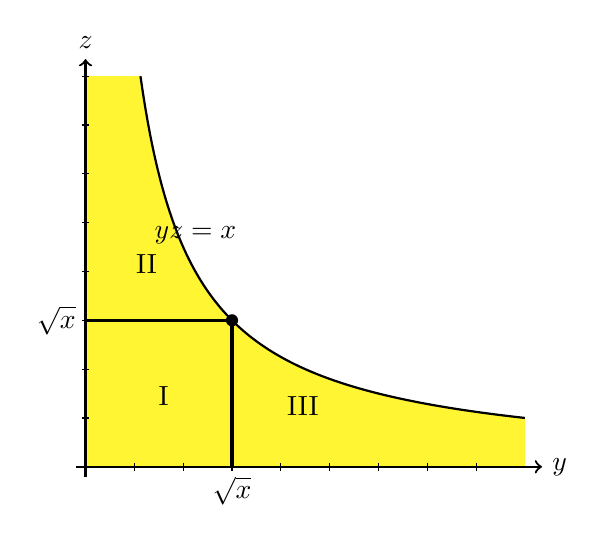
\begin{tikzpicture}[x=0.62cm,y=0.62cm]
  % The scale is normalized so that sqrt(x)=3 and hence yz=x is z=9/y.
  \begin{scope}
    \clip (0,0) rectangle (9,8);
    \fill[yellow!80] (0,0) -- (0,8) -- (1.125,8) --
      plot[domain=1.125:9,samples=160] (\x,{9/\x}) -- (9,0) -- cycle;
  \end{scope}
  \draw[->,thick] (-0.2,0) -- (9.35,0) node[right] {$y$};
  \draw[->,thick] (0,-0.2) -- (0,8.35) node[above] {$z$};
  \foreach \t in {1,...,8}{
    \draw (\t,0.08) -- (\t,-0.08);
    \draw (0.08,\t) -- (-0.08,\t);
  }
  \draw[very thick] (0,3) -- (3,3) -- (3,0);
  \draw[thick,domain=1.125:9,samples=160] plot (\x,{9/\x});
  \fill (3,3) circle[radius=2.2pt];
  \node at (1.6,1.45) {I};
  \node at (1.25,4.15) {II};
  \node at (4.45,1.25) {III};
  \node at (2.25,4.75) {$yz=x$};
  \node[left] at (0,3) {$\sqrt{x}$};
  \node[below] at (3,0) {$\sqrt{x}$};
\end{tikzpicture}
\caption{The Dirichlet divisor problem.}
\label{fig:divisor-problem}
\end{figure}

fractional part of $x$, as $x \to \infty$,

$$
\begin{aligned}
D(x) & =\sum_{d \leq x}\floor{\frac{x}{d}}=\sum_{d \leq \sqrt{x}}\floor{\frac{x}{d}}+\sum_{d \leq \sqrt{x}}\floor{\frac{x}{d}}-\floor{\sqrt{x}}^{2} \\
& =2 \sum_{d \leq \sqrt{x}}\left(\frac{x}{d}+O(1)\right)-(\sqrt{x}-\{\sqrt{x}\})^{2} \\
& =2 x \sum_{d \leq \sqrt{x}} \frac{1}{d}+O(\sqrt{x})-x+O(\sqrt{x}) \\
& =2 x(\log \sqrt{x}+\gamma+O(1 / \sqrt{x}))-x+O(\sqrt{x}) \\
& =x \log x+(2 \gamma-1) x+O(\sqrt{x}),
\end{aligned}
$$

where in the penultimate step we used a familiar estimate for a partial sum of the harmonic series [32, p. 99], i.e.,

$$
\sum_{n \leq x} \frac{1}{n}=\log x+\gamma+O\left(\frac{1}{x}\right) .
$$
\end{proof}

In deriving the first improvement on Dirichlet's upper bound for $\Delta(x)$, in 1904, Voronoï employed the summation formula named after him and proved that [39]


\begin{equation*}
\Delta(x)=O\left(x^{1 / 3} \log x\right), \quad x \to \infty . \tag{3.3}
\end{equation*}


In analogy to the formula of Ramanujan, Hardy, and Landau (2.4), Voronoï [39] established a representation for $\Delta(x)$ in terms of Bessel functions. To state this representation, we need to recall the definitions of the Bessel function $Y_{\nu}(z)$ of the second kind [40, p.~64, equation (1)]


\begin{equation*}
Y_{\nu}(z):=\frac{J_{\nu}(z) \cos (\nu\pi)-J_{-\nu}(z)}{\sin (\nu\pi)}, \tag{3.4}
\end{equation*}


and the modified Bessel function $K_{\nu}(z)$, [40, p. 78, equation (6)], for $-\pi<\arg z<\frac{\pi}{2}$,


\begin{equation*}
K_{\nu}(z):=\frac{\pi}{2} \frac{e^{\pi i\nu / 2} J_{-\nu}(i z)-e^{-\pi i\nu / 2} J_{\nu}(i z)}{\sin (\nu\pi)} . \tag{3.5}
\end{equation*}


If $\nu$ is an integer $n$, it is understood that we define the functions by taking the limits as $\nu \to n$ in (3.4) and (3.5). We can now state Voronoï's formula,


\begin{equation*}
\sum_{n \leq x}^{\prime} d(n)=x(\log x+2 \gamma-1)+\frac{1}{4}+\sum_{n=1}^{\infty} d(n)\left(\frac{x}{n}\right)^{1 / 2} I_{1}(4 \pi \sqrt{n x}) \tag{3.6}
\end{equation*}


where $x>0$, $\gamma$ denotes Euler's constant, and $I_{1}(z)$ is defined by


\begin{equation*}
I_{\nu}(z):=-Y_{\nu}(z)-\frac{2}{\pi} K_{\nu}(z) . \tag{3.7}
\end{equation*}


(Note the aforementioned appearance of the term $+\frac{1}{4}$ in (3.6).) As $x \to \infty$ [40, pp. 199, 202],

% The standard phase in the Y_nu asymptotic is x-pi*nu/2-pi/4;
% the printed article has pi*nu/4.
\begin{gather*}
Y_{\nu}(x)=\sqrt{\frac{2}{\pi x}} \sin \left(x-\frac{\pi\nu}{2}-\frac{\pi}{4}\right)+O\left(\frac{1}{x^{3 / 2}}\right)  \tag{3.8}\\
K_{\nu}(x)=\sqrt{\frac{\pi}{2 x}} e^{-x}+O\left(e^{-x} \frac{1}{x^{3 / 2}}\right) \tag{3.9}
\end{gather*}


Comparing the asymptotic formulas (3.8), (3.9), and (2.3), we conclude, as before, that the series on the right-hand side of (3.6) converges conditionally but not absolutely. Since the establishment of (3.6) in 1904, Voronoï's formula has been the starting point for most attempts at finding an upper bound for $\Delta(x)$.

We briefly remark that the circle problem can be generalized to higher-dimensional ellipsoids, and the divisor problem can be generalized to larger numbers of divisors. Perhaps Landau [24] was the first to generalize Sierpiński's and Voronoï's theorems in these directions. Because a worthy discussion of these generalizations would considerably lengthen this paper, we shall not write anything further about them.

\section{Upper Bounds for \texorpdfstring{$P(x)$ and $\Delta(x)$}{P(x) and Delta(x)}}

The histories of establishing upper and lower bounds for $P(x)$ and $\Delta(x)$ are similar. If an upper bound is obtained for $P(x)$, then usually the same method applies to $\Delta(x)$ to obtain a similar upper bound, and conversely. Many of these upper bounds for $P(x)$ and $\Delta(x)$ involve logarithms or iterated logarithms, which we ignore in our brief survey. Thus, let us set $P(x)=O\left(x^{a+\epsilon}\right)$ $\left(\Delta(x)=O\left(x^{a+\epsilon}\right)\right)$, for every $\epsilon>0$, and record some of the values of $a$ that have been obtained during the past century or more.

\begin{center}
\small
\begin{tabular}{@{}ll@{}}
\toprule
Exponent & Mathematician(s) and year \\
\midrule
$a=1/2$ & Gauss ($\approx1800$), Dirichlet (1849) \\
$a=1/3$ & Voronoï (1904), Sierpiński (1906), Landau (1913) \\
$a=33/100$ & van der Corput (1923) \\
$a=37/112=0.3303\ldots$ & Littlewood and Walfisz (1924), Hardy (1925) \\
$a=163/494=0.3299\ldots$ & Walfisz (1927) \\
$a=27/82=0.3292\ldots$ & van der Corput (1928), Nieland (1928) \\
$a=15/46=0.3260\ldots$ & Titchmarsh (1934), Chih (1950), Richert (1953) \\
$a=13/40=0.3250\ldots$ & Hua (1942) \\
$a=12/37=0.3243\ldots$ & Chen (1963), Kolesnik (1969) \\
$a=346/1067=0.3242\ldots$ & Kolesnik (1973) \\
$a=35/108=0.324074\ldots$ & Kolesnik (1982) \\
$a=139/429=0.324009\ldots$ & Kolesnik (1985) \\
$a=7/22=0.3181\ldots$ & Iwaniec and Mozzochi (1988) \\
$a=23/73=0.3150\ldots$ & Huxley (1993) \\
$a=131/416=0.3149\ldots$ & Huxley (2003) \\
\bottomrule
\end{tabular}
\end{center}

Complete citations for the results quoted above can be found in our list of references at the end of this paper. In summary, in about 100 years, the exponents on Sierpiński's and Voronoï's upper bounds have been improved by slightly less than 0.02.

We now offer a few words about how upper bounds have been obtained. Although (3.6) is an exact formula, in applications to the divisor problem, we use the asymptotic formulas (3.8) and (3.9) and truncate the series, where the upper bound of the truncated series and the error made may depend upon several parameters. An excellent source to learn such methods is Titchmarsh's classic text [35, Chapter 12]. For example, if $\zeta(s)$ denotes the Riemann zeta function and $\zeta(s) x^{s} / s$ is integrated over a rectangle with vertices $-a-i T, c-i T, c+i T,-a+i T$, then [35, p. 319, equation (12.4.3)]


\begin{align*}
\Delta(x)= & \frac{x^{1 / 4}}{\pi \sqrt{2}} \sum_{n \leq N} \frac{d(n)}{n^{3 / 4}} \cos \left(4 \pi \sqrt{n x}-\frac{1}{4} \pi\right) \\
& +O\left(x^{-1 / 4}\right)+O\left(\frac{T^{2 a}}{x^{a}}\right)+O\left(\frac{x^{c}}{T}\right), \tag{4.1}
\end{align*}


% ed.: the printed citation [38] for van der Corput's 27/82 is his 1923 paper, which gives 33/100 (see the table);
% the bound 27/82 is from van der Corput, Zum Teilerproblem, Math. Ann. 98 (1928) 697-716, not in the reference list.
where $N+\frac{1}{2}=T^{2} /\left(4 \pi^{2} x\right)$. (Of course, a similar remark can be made for (2.4).) Titchmarsh uses (4.1) to obtain the bound $\frac{27}{82}$ established by L. W. Nieland [31] and J. G. van der Corput [38]. This, or a similar, truncated formula (4.1) has been the starting point for most attacks on the error term $\Delta(x)$.

% ed.: printed text cites [23] (Pacific J. Math. 98, 1982, exponent 35/108) for the 1985 result 139/429;
% the 1985 paper is Kolesnik, On the method of exponent pairs, Acta Arith. 45 (1985) 115-143, not in the reference list.
Approximating $\Delta(x)$ by double exponential sums with the use of Voronoï's formula (3.6), as we did above in (4.1), was accomplished with great success by many mathematicians listed in our table, up to and including G. A. Kolesnik in his 1985 paper [23], where he uses the van der Corput method to estimate trigonometric sums of several variables.

H. Iwaniec and C. J. Mozzochi [22] use a variety of methods related to Farey fractions and Weyl and van der Corput's treatment of exponential sums, but their main, new source of inspiration was provided by the work of E. Bombieri and H. Iwaniec [9]. In this pioneering work, among other things, Bombieri and Iwaniec examine certain averages of exponential sums by methods of Weyl and van der Corput, but they first analyze and transform these sums before averaging. Via an approximation by a cubic Taylor polynomial, they arrive at certain perturbed Gauss sums. They then can transform these by using the Poisson summation formula.

M. N. Huxley in 1993 [18], and then again in 2003 [19], succeeded in improving previous results via a refinement of the methods of Iwaniec and Mozzochi, with one of his main ingredients being an estimate for the number of lattice points close to a smooth curve due to himself [20].

\section{Lower Bounds for \texorpdfstring{$P(x)$ and $\Delta(x)$}{P(x) and Delta(x)}}

% ed.: printed text has [16, pp. 243-267]; corrected to 243-263, consistent with Section 2, with [16, p. 263] in Section 5, and with the 21-page original [14, pp. 263-283].
It is natural to ask if lower bounds for $P(x)$ can be obtained. Landau [28] and Hardy [14], [16, pp. 243-263] in papers both published in 1915, obtained the first results in this direction. Employing an identity for the ``smoothed'' sum

% As in (2.5), the printed lower limit n=0 is incompatible with the factor x/n.
$$
\sum_{0 \leq n \leq x} r_{2}(n)(x-n)=\frac{\pi x^{2}}{2}+\frac{1}{\pi} \sum_{n=1}^{\infty} r_{2}(n)\frac{x}{n} J_{2}(2 \pi \sqrt{n x}),
$$

Landau [28] showed that for every $\epsilon>0, P(x) \neq O\left(x^{1 / 4-\epsilon}\right)$, as $x \to \infty$.

To describe Hardy's theorems, recall the definitions of $f(x)=\Omega(F(x)), f(x)=\Omega_{+}(F(x)), f(x)=\Omega_{-}(F(x))$, and $f(x)=\Omega_{ \pm}(F(x))$, as $x \to \infty$, which we made at the close of the Introduction.

% ed.: printed text has [16, pp. 243-267]; corrected to 243-263 (see the note in the first paragraph of this section).
Improving on Landau's result, but using a completely different method, Hardy [14], [16, pp. 243-263] proved that


\begin{equation*}
P(x)=\Omega_{ \pm}\left(x^{1 / 4}\right), \quad \text { as } x \to \infty . \tag{5.1}
\end{equation*}


Shortly thereafter, Hardy [15], [16, pp. 268-292] obtained an analog of (5.1) for $\Delta(x)$ and then improved (5.1) by showing that


\begin{equation*}
P(x)=\Omega_{-}\left(\{x \log x\}^{1 / 4}\right), \quad \text { as } x \to \infty . \tag{5.2}
\end{equation*}


Hardy's result for $\Delta(x)$ is slightly better than that for $P(x)$. In particular, Hardy [15], [16, pp. 268-292] proved that


\begin{equation*}
\Delta(x)=\Omega_{+}\left(\{x \log x\}^{1 / 4} \log \log x\right) . \tag{5.3}
\end{equation*}


After the theorems of Hardy, progress toward obtaining improved lower bounds has been slow. The table below records improvements that have been made since 1916. Complete bibliographic details can be found in our list of references.

$$
P(x)=\Omega_{ \pm}\left(x^{1 / 4}(\log \log x)^{1 / 4}(\log \log \log x)^{1 / 4}\right)
$$

Gangadharan (1961)

$$
P(x)=\Omega_{+}\left(x^{1 / 4} \exp \left(C_{1}(\log \log x)^{1 / 4}(\log \log \log x)^{-3 / 4}\right)\right)
$$

Corrádi and Kátai (1967)

$$
P(x)=\Omega_{-}\left(x^{1 / 4}(\log x)^{1 / 4}(\log \log x)^{(\log 2) / 4} \exp \left(-C_{2} \sqrt{\log \log \log x}\right)\right)
$$

Hafner (1981)

$$
P(x)=\Omega\left(x^{1 / 4}(\log x)^{1 / 4} \frac{(\log \log x)^{3\left(2^{1 / 3}-1\right) / 4}}{(\log \log \log x)^{5 / 8}}\right)
$$

Soundararajan (2003).

Here, $C_{1}$ and $C_{2}$ are certain positive constants. We note in passing that A. Selberg had previously obtained Hafner's result but did not publish it. In 1974, Selberg communicated his improvements to the first author, who later passed them to his doctoral student, J. L. Hafner, along with a sentence from Selberg indicating his primary idea in improving Hardy's $\Omega$-theorem. The exponents of $\log \log x$ in the last two $\Omega$-theorems are

$$
\frac{1}{4} \log 2=0.1732 \ldots \quad \text { and } \quad \frac{3\left(2^{1 / 3}-1\right)}{4}=0.1949 \ldots .
$$

We emphasize that analogous $\Omega$-theorems hold for $\Delta(x)$.

Most number theorists who have thought about the circle problem and the divisor problem think that the foregoing results are closer to the truth than the upper bounds that have been obtained. In fact, it is conjectured that


\begin{equation*}
P(x)=O\left(x^{1 / 4+\epsilon}\right), \quad \Delta(x)=O\left(x^{1 / 4+\epsilon}\right), \quad x \to \infty, \quad \text { for every } \epsilon>0 . \tag{5.4}
\end{equation*}


Bounds for $P(x)$ and $\Delta(x)$ frequently lead to analogous improved upper bounds for $\zeta\left(\frac{1}{2}+i t\right)$, as $|t| \to \infty$. Thus, two of the most significant and difficult problems in number theory, perhaps rivaling the Lindelöf hypothesis, namely, $\zeta\left(\frac{1}{2}+i t\right)=O\left(|t|^{\epsilon}\right)$, as $|t| \to \infty$, in difficulty, are the conjectures (5.4).

We observe that Hardy's result (5.3) is better on the plus side than what he and others have been able to obtain on the minus side. One might therefore conjecture that $\Delta(x)$ is more often positive than negative. Indeed, it is a consequence of Voronoï's work [39] that

$$
\int_{0}^{X} \Delta(x) d x=\frac{1}{4} X+O\left(X^{3 / 4}\right), \quad X \to \infty .
$$

Thus, indeed, $\Delta(x)$ is more frequently positive than negative.

On the other hand, Hardy's $\Omega$-theorem (5.2) and Hafner's improvement [13] point to a possibly negative bias of values for $P(x)$. Indeed, for $m=3,4$, K.-M. Tsang [36], and, for $5 \leq m \leq 9$, W. Zhai [41] showed that

$$
\int_{0}^{X} P^{m}(x) d x \sim(-1)^{m} C_{m} X^{1+m / 4}, \quad X \to \infty ,
$$

where $C_{m}>0$ and $3 \leq m \leq 9$. Thus, $P(x)$ prefers to be negative.

In his paper [14], Hardy related a beautiful identity of Ramanujan connected with $r_{2}(n)$, namely, for $a, b>0$, [14, p. 283], [16, p. 263],


\begin{equation*}
\sum_{n=0}^{\infty} \frac{r_{2}(n)}{\sqrt{n+a}} e^{-2 \pi \sqrt{(n+a) b}}=\sum_{n=0}^{\infty} \frac{r_{2}(n)}{\sqrt{n+b}} e^{-2 \pi \sqrt{(n+b) a}}, \tag{5.5}
\end{equation*}


which is not given elsewhere in any of Ramanujan's published or unpublished work. Observe the beautiful symmetry of $a$ and $b$ in (5.5). If we differentiate (5.5) with respect to $b$, let $a \to 0$, replace $2 \pi \sqrt{b}$ by $s$, and use analytic continuation, we find that, for $\operatorname{Re}(s)>0$,

$$
\sum_{n=1}^{\infty} r_{2}(n) e^{-s \sqrt{n}}=\frac{2 \pi}{s^{2}}-1+2 \pi s \sum_{n=1}^{\infty} \frac{r_{2}(n)}{\left(s^{2}+4 \pi^{2} n\right)^{3 / 2}},
$$

which was the key identity in Hardy's proof of (5.1).

\section{Further Evidence of Ramanujan's Strong Interest in the Circle and Divisor Problems}

Recall that Ramanujan was in Cambridge with Hardy during the years 1914--1919. Hardy's two papers [14] and [15] on the circle and divisor problems were published in 1915 and 1916, respectively. In the foregoing passages, we have noted two instances when Ramanujan and Hardy clearly communicated with each other about the circle problem. Published with Ramanujan's lost notebook is a page [33, p. 335] that provides further evidence that Ramanujan had a keen interest in both the circle and divisor problems. Page 335 is, in fact, not a page in the original lost notebook found at Trinity College Library, Cambridge by George Andrews in March, 1976. (For an excellent account of his discovery, see Andrews's Monthly paper [1] as well as his more up-to-date account [2].) Published with the lost notebook are several fragments and partial manuscripts written by Ramanujan, and page 335 is one of these fragments. In the remainder of this section, we focus on the identity on page 335 that is associated with the circle problem. Ramanujan recorded an analogous identity associated with the divisor problem.

To motivate Ramanujan's first identity, we begin by recalling Jacobi's formula [4, p. 56, Theorem 3.2.1]


\begin{equation*}
r_{2}(n)=4 \sum_{\substack{d \mid n \\ d \text { odd }}}(-1)^{(d-1) / 2}, \tag{6.1}
\end{equation*}


for all positive integers $n$. To encode the endpoint convention represented by the prime on a summation sign, let $F$ be the endpoint-weighted floor function defined in (6.3) below. We can then recast (2.4) in the form, for $x>0$,


% In the printed last line of (6.2), a primed d-sum with floor(x/d)
% fails to half-weight every boundary pair dj=x. The function F(x/d) does so exactly.
\begin{align*}
\pi x-1+\sum_{n=1}^{\infty} r_{2}(n)\left(\frac{x}{n}\right)^{1 / 2} J_{1}(2 \pi \sqrt{n x}) & =\sum_{0<n \leq x}^{\prime} r_{2}(n) \\
& =4 \sum_{0<n \leq x}^{\prime} \sum_{d \mid n} \sin \left(\frac{\pi d}{2}\right) \\
& =4 \sum_{0<d j \leq x}^{\prime} \sin \left(\frac{\pi d}{2}\right) \\
& =4 \sum_{0<d \leq x}F\left(\frac{x}{d}\right) \sin \left(\frac{\pi d}{2}\right). \tag{6.2}
\end{align*}


Explicitly, the function required in (6.2) and in Ramanujan's first claim on page 335 of [33] is

\begin{equation*}
F(x)=
\begin{cases}
\floor{x}, & \text{if $x$ is not an integer},\\
x-\dfrac{1}{2}, & \text{if $x$ is an integer}.
\end{cases}
\tag{6.3}
\end{equation*}

\begin{entry}[{\normalfont [33, p.~335]}]
Let $F(x)$ be defined by (6.3), and recall that $J_{1}(z)$ is defined in (2.2). If $0<\theta<1$ and $x>0$, then


\begin{align*}
& \sum_{n=1}^{\infty} F\left(\frac{x}{n}\right) \sin (2 \pi n \theta)=\pi x\left(\frac{1}{2}-\theta\right)-\frac{1}{4} \cot (\pi \theta)  \tag{6.4}\\
& \quad+\frac{1}{2} \sqrt{x} \sum_{m=1}^{\infty} \sum_{n=0}^{\infty}\left\{\frac{J_{1}(4 \pi \sqrt{m(n+\theta) x})}{\sqrt{m(n+\theta)}}-\frac{J_{1}(4 \pi \sqrt{m(n+1-\theta) x})}{\sqrt{m(n+1-\theta)}}\right\} .
\end{align*}
\end{entry}

As we shall see in the sequel, there is some evidence that Ramanujan did not intend the double sum in (6.4) to be interpreted as an iterated sum, but as a double sum in which the product $mn$ of the summation indices tends to $\infty$.

Note that the series on the left-hand side of (6.4) is finite, and discontinuous if $x$ is an integer. We also observe that there are singularities at $\theta=0$ and $\theta=1$ on the right-hand side, but if (6.4) is true, then these singularities cancel each other out. To examine the convergence of the series on the right-hand side of (6.4), we recall (2.3). Hence, as $m, n \to \infty$, the terms of the double series on the right-hand side of (6.4) are asymptotically equal to

$$
\begin{aligned}
\frac{1}{\pi \sqrt{2} x^{1 / 4} m^{3 / 4}} & \left(\frac{\cos \left(4 \pi \sqrt{m(n+\theta) x}-\frac{3}{4} \pi\right)}{(n+\theta)^{3 / 4}}\right. \\
& \left.-\frac{\cos \left(4 \pi \sqrt{m(n+1-\theta) x}-\frac{3}{4} \pi\right)}{(n+1-\theta)^{3 / 4}}\right) .
\end{aligned}
$$

Thus, if indeed the double series on the right-hand side of (6.4) does converge, it converges conditionally and not absolutely.

Noting the definition (6.3), compare (6.4) with the equality from the extremal sides of (6.2) and observe the close resemblance. Thus, it seems plausible that there is a connection between these two formulas, which we shall indeed demonstrate. Ramanujan might therefore have derived (6.4) in anticipation of applying it to the circle problem. Often, in analysis, when an extra parameter is introduced, it opens up new attacks on a problem, but if Ramanujan had such ideas, they have remained hidden to us for nearly a century.

Entry 3 was first proved by B. C. Berndt and A. Zaharescu [8] with the order of summation on the double sum reversed from that recorded by Ramanujan. The authors of [8] were able to prove this emended version of Ramanujan's claim by first replacing Entry 3 with the following equivalent theorem.

\begin{theorem}
For $0<\theta<1$ and $x>0$,


\begin{align*}
& \sum_{n=1}^{\infty} F\left(\frac{x}{n}\right) \sin (2 \pi n \theta)-\pi x\left(\frac{1}{2}-\theta\right) \\
& \quad=\frac{1}{\pi} \sum_{n=0}^{\infty} \sum_{m=1}^{\infty}\left(\frac{1}{n+\theta} \sin ^{2}\left(\frac{\pi(n+\theta) x}{m}\right)-\frac{1}{n+1-\theta} \sin ^{2}\left(\frac{\pi(n+1-\theta) x}{m}\right)\right) . \tag{6.5}
\end{align*}
\end{theorem}

It should be emphasized that this reformulation fails to exist for Ramanujan's original formulation in Entry 3, with the order of summation reversed from that in (6.5). After proving the aforementioned alternative version of Entry 3, the authors of [8] derived an identity involving the twisted character sums


\begin{equation*}
d_{\chi}(n)=\sum_{k \mid n} \chi(k), \tag{6.6}
\end{equation*}


where $\chi$ is an odd primitive character modulo $q$. We do not state this identity here, but using it, the authors of [8] derived a representation for $\sump_{0 \leq n \leq x} r_{2}(n)$.

\begin{corollary}
For any $x>0$,


\begin{align*}
\sump_{0\leq n\leq x} r_{2}(n)
={}&\pi x+2\sqrt{x}\sum_{n=0}^{\infty}\sum_{m=1}^{\infty}
\Biggl\{
\frac{J_{1}\!\left(4\pi\sqrt{m\left(n+\frac14\right)x}\right)}
     {\sqrt{m\left(n+\frac14\right)}} \\
&\hspace{4.8cm}{}-
\frac{J_{1}\!\left(4\pi\sqrt{m\left(n+\frac34\right)x}\right)}
     {\sqrt{m\left(n+\frac34\right)}}
\Biggr\}.
\tag{6.7}
\end{align*}
\end{corollary}


The summands in (6.7) have a remarkable resemblance to those in the original identity (6.2) of Ramanujan, Hardy, and Landau. It is therefore natural to ask if the two identities are equivalent. Berndt, S. Kim, and Zaharescu [5] proved that (6.2) (or (2.4)) and (6.7) are versions of the same identity, provided that a certain rearrangement of the double series in (6.7) is justified, namely, that the product of the indices $mn$ tends to infinity, i.e., $m$ and $n$ are tending to infinity ``together.'' In view of these comments, we might conjecture that, although Ramanujan wrote the right-hand side of (6.4) as an iterated double sum, he possibly had derived (6.4) under the assumption that the product of the indices $mn$ tends to infinity. Therefore, a proof of (6.4) with this method of summation being assumed was provided [5].

Finally, in [6], (6.4) was established with the order of summation on the right-hand side of (6.4) as prescribed by Ramanujan.

In summary, Entry 3 has been proved under three different assumptions on the order of summation for the double series on the right-hand side of (6.4). The three proofs are entirely different; nothing from one proof is used in any of the other two proofs. As we mentioned earlier, the first proof that was given depends upon initially establishing the equivalent Theorem 4. The proof of Entry 3 under the assumption that the product of the indices tends to infinity eventually rests upon a much earlier delicate Fourier analysis by K. Chandrasekharan and R. Narasimhan [10] and an identity for the summatory function of weighted divisors (6.6) for odd primitive characters in [3, Theorem 2]. The proof of Entry 3 under Ramanujan's original formulation is the most difficult of all three (difficult) proofs. The aforementioned authors begin with the asymptotic formula (2.3), but the resulting double sum must be subdivided into several subintervals in order to show that it converges uniformly on compact subsets of $0<\theta<1$ and that the right-hand side of (6.4) is a continuous function at $\theta=0$ and $\theta=1$. New methods for estimating trigonometric sums were introduced in this proof of Ramanujan's claim. More precisely, in some ranges, better than square root cancellation is achieved by breaking the sums into even smaller ranges where the functions appearing in those exponentials are almost linear. This proved to be essential in the process of obtaining enough cancellation to successfully complete the proof of Ramanujan's claim. It is plausible that these methods and techniques employed in the proof of Ramanujan's claim will be useful to researchers in the future.

\section{Concluding Remarks}

The circle and divisor problems are intimately connected with several further important unsolved problems in number theory. We cite one such problem that is closely connected to the previously mentioned Lindelöf hypothesis. Hardy and Littlewood showed in 1918 that [17], [16, pp. 20-97]


\begin{equation*}
\int_{0}^{T}\left|\zeta\left(\frac{1}{2}+i t\right)\right|^{2} d t=T \log \frac{T}{2 \pi}+(2 \gamma-1) T+E(T) \tag{7.1}
\end{equation*}


where $\zeta(s)$ denotes the Riemann zeta-function and the error term $E(T)=o(T \log T)$, as $T \to \infty$. Many mathematicians have derived improved bounds for $E(T)$, and the precise order of $E(T)$ is unknown. Furthermore, if $N$ is approximately equal to $T$, then the primary contribution to the error term $E(T)$ has the shape


\begin{equation*}
\left(\frac{2 T}{\pi}\right)^{1 / 4} \sum_{n \leq N}(-1)^{n} \frac{d(n)}{n^{3 / 4}} \cos \left(2 \sqrt{2 \pi n T}-\frac{1}{4} \pi\right) . \tag{7.2}
\end{equation*}


Readers should compare (7.2) with (4.1). Therefore, not surprisingly, an improved estimate for $\Delta(x)$ invariably leads to an improved estimate for $E(T)$, and conversely.

We have discussed the number of lattice points in two particular planar regions, the circle and the first quadrant under a hyperbola. Number theorists have examined similar problems for many other regions in spaces of arbitrary dimensions, including $n$-dimensional spheres. For excellent, but more technical, survey articles on many unsolved problems on divisor sums, lattice sums, the Riemann zeta-function, in particular, the Lindelöf hypothesis, abelian groups, and further related topics, the authors highly recommend the survey papers by K.-M. Tsang [37] and by A. Ivić, E. Krätzel, M. Kühleitner, and W. G. Nowak [21]. A more technical survey paper emphasizing Ramanujan's intriguing formulas connected with the circle and divisor problems was written for the 125th anniversary of Ramanujan's birth [7].

\section*{Acknowledgment}
The authors thank Byungchan Kim for the two geometrical figures appearing in this paper.

\section*{References}
\begin{list}{}{\setlength{\leftmargin}{2.7em}\setlength{\labelwidth}{2.2em}\setlength{\itemindent}{-2.7em}\setlength{\itemsep}{0.25ex}\small}
  \item[{[1]}] Andrews, G. E. (1979). An introduction to Ramanujan's ``lost'' notebook. Amer. Math. Monthly. 86: 89-108.
  \item[{[2]}] Andrews, G. E. (2013). The discovery of Ramanujan's lost notebook. In: Berndt, B. C., Prasad, D., eds. The Legacy of Srinivasa Ramanujan: Proceedings of an International Conference in Celebration of the 125th Anniversary of Ramanujan's Birth: University of Delhi, 17-22 December 2012. Mysore: Ramanujan Mathematical Society, pp. 77-88.
  \item[{[3]}] Berndt, B. C. (1969). Identities involving the coefficients of a class of Dirichlet series. I. Trans. Amer. Math. Soc. 137: 345-359.
  \item[{[4]}] Berndt, B. C. (2006). Number Theory in the Spirit of Ramanujan. Providence, RI: American Mathematical Society.
  \item[{[5]}] Berndt, B. C., Kim, S., Zaharescu, A. (2012). Weighted divisor sums and Bessel function series, II. Adv. Math. 229: 2055-2097.
  \item[{[6]}] Berndt, B. C., Kim, S., Zaharescu, A. (2013). The circle and divisor problems, and double series of Bessel functions. Adv. Math. 236: 24-59.
  \item[{[7]}] Berndt, B. C., Kim, S., Zaharescu, A. (2013). The circle and divisor problems, and Ramanujan's contributions through Bessel function series. In: Berndt, B. C., Prasad, D., eds. The Legacy of Srinivasa Ramanujan: Proceedings of an International Conference in Celebration of the 125th Anniversary of Ramanujan's Birth: University of Delhi, 17-22 December 2012. Mysore: Ramanujan Mathematical Society, pp. 111-127.
  \item[{[8]}] Berndt, B. C., Zaharescu, A. (2006). Weighted divisor sums and Bessel function series. Math. Ann. 335: 249-283.
  \item[{[9]}] Bombieri, E., Iwaniec, H. (1986). Some mean-value theorems for exponential sums. Ann. Scuola Norm. Sup. Pisa Cl. Sci. 13(3): 473-486.
  \item[{[10]}] Chandrasekharan, K., Narasimhan, R. (1961). Hecke's functional equation and arithmetical identities. Ann. Math. 74: 1-23.
  \item[{[11]}] Dirichlet, J. G. L. (1849). Über die Bestimmung der mittleren Werthe in der Zahlentheorie. Abh. K. Akad. Wiss. Berlin 1849: 69-83.
  \item[{[12]}] Gauss, C. F. (1876). De nexu inter multitudinem classium, in quas formae binariae secundi gradus distribuuntur, earumque determinantem. In: Schering, E., ed., Werke, Vol. 2. Göttingen: Königlichen Gesellschaft der Wissenschaften, pp. 269-291.
\end{list}

\begin{list}{}{\setlength{\leftmargin}{2.7em}\setlength{\labelwidth}{2.2em}\setlength{\itemindent}{-2.7em}\setlength{\itemsep}{0.25ex}\small}
  \item[{[13]}] Hafner, J. L. (1981). New omega theorems for two classical lattice point problems. Invent. Math. 63: 181-186.
  \item[{[14]}] Hardy, G. H. (1915). On the expression of a number as the sum of two squares. Quart. J. Math. (Oxford). 46: 263-283.
  \item[{[15]}] Hardy, G. H. (1916). On Dirichlet's divisor problem. Proc. London Math. Soc. 15: 1-25.
  \item[{[16]}] Hardy, G. H. (1967). Collected Papers. Vol. II. Oxford: The Clarendon Press, Oxford University Press.
  \item[{[17]}] Hardy, G. H., Littlewood, J. E. (1918). Contributions to the theory of the Riemann zeta-function and the theory of the distribution of primes. Acta Math. 41: 119-196.
  \item[{[18]}] Huxley, M. N. (1993). Exponential sums and lattice points. I. Proc. London Math. Soc. 66: 279-301.
  \item[{[19]}] Huxley, M. N. (2003). Exponential sums and lattice points. III. Proc. London Math. Soc. 87: 591-609.
  \item[{[20]}] Huxley, M. N. (1999). The integer points close to a curve. III. In: Number Theory in Progress. Vol. 2 (Zakopane--Kościelisko, 1997). Berlin: de Gruyter, pp. 911-940.
  \item[{[21]}] Ivić, A., Krätzel, E., Kühleitner, M., Nowak, W. G. (2006). Lattice points in large regions and related arithmetic functions: Recent developments in a very classic topic. In: Schwarz, W., Steuding, J., eds., Proc. ELAZ-Conf., May 24-28, 2004. Stuttgart: Franz Steiner Verlag, pp. 89-128.
  \item[{[22]}] Iwaniec, H., Mozzochi, C. J. (1988). On the divisor and circle problems. J. Number Theory 29: 60-93.
  \item[{[23]}] Kolesnik, G. A. (1982). On the order of $\zeta(1 / 2+i t)$ and $\Delta(R)$. Pacific J. Math. 98: 107-122.
  \item[{[24]}] Landau, E. (1912). Über die Anzahl der Gitterpunkte in gewissen Bereichen. Göttingen: Nachr. Akad. Wiss., pp. 687-771.
  \item[{[25]}] Landau, E. (1913). Über einen Satz des Herrn Sierpiński. Giornale di Matematiche di Battaglini. 51: 73-81.
  \item[{[26]}] Landau, E. (1913). Über die Zerlegung der Zahlen in zwei Quadrate. Annali di Matematica Pura ed Applicata (3) 20: 1-28.
  \item[{[27]}] Landau, E. (1915). Über die Gitterpunkte in einem Kreise (Erste Mitteilung). Göttingen: Nachr. Akad. Wiss., pp. 148-160.
  \item[{[28]}] Landau, E. (1915). Über die Gitterpunkte in einem Kreise (Zweite Mitteilung). Göttingen: Nachr. Akad. Wiss., pp. 161-171.
  \item[{[29]}] Landau, E. (1947). Zahlentheorie, Zweiter Band, Vorlesungen über Zahlentheorie. New York: Chelsea.
  \item[{[30]}] Littlewood, J. E., Walfisz, A. (1924). The lattice points of a circle. Proc. Roy. Soc. (A). 106: 478-488.
  \item[{[31]}] Nieland, L. W. (1928). Zum Kreisproblem. Math. Ann. 98: 717-736.
  \item[{[32]}] Rademacher, H. (1964). Lectures on Elementary Number Theory. New York: Blaisdell.
  \item[{[33]}] Ramanujan, S. (1988). The Lost Notebook and Other Unpublished Papers. New Delhi: Narosa.
  \item[{[34]}] Sierpiński, W. (1906). O pewnem zagadnieniu z rachunku funkcyj asymptotycznych. Prace Mat. Fiz. 17: 77-118.
  \item[{[35]}] Titchmarsh, E. C. (1986). The Theory of the Riemann Zeta-Function. 2nd ed. Oxford: The Clarendon Press, Oxford Univ. Press.
  \item[{[36]}] Tsang, K.-M. (1992). Higher-power moments of $\Delta(x), E(t)$ and $P(x)$. Proc. London Math. Soc. 65: 65-84.
  \item[{[37]}] Tsang, K.-M. (2010). Recent progress on the Dirichlet divisor problem and the mean square of the Riemann zeta-function. Sci. China Mathematics. 53(9): 2561-2572.
  \item[{[38]}] van der Corput, J. G. (1923). Neue zahlentheoretische Abschätzungen. Math. Ann. 89: 215-254.
  \item[{[39]}] Voronoï, G. F. (1904). Sur une fonction transcendante et ses applications à la sommation de quelques séries. Ann. École Norm. Sup. 21: 207-267, 459-533.
  \item[{[40]}] Watson, G. N. (1966). Theory of Bessel Functions. 2nd ed. Cambridge: Cambridge Univ. Press.
  \item[{[41]}] Zhai, W. (2004). On the higher-power moments of $\Delta(x)$ (II). Acta Arith. 114: 35-54.
\end{list}

\paragraph{Bruce C. Berndt.} Since 1974, he has devoted almost all of his research to the mathematics of India's greatest mathematician, Srinivasa Ramanujan. Most of his 37 current and former doctoral students, several postdoctorates, and the co-authors of this paper have greatly aided him in this endeavor. He has published 12 books on the mathematics and life of Ramanujan. Berndt and George Andrews are currently completing their fifth and last book on Ramanujan's lost notebook. This is the eleventh article that Berndt has published in the American Mathematical Monthly, two of which have received awards.

Department of Mathematics, University of Illinois, 1409 West Green Street, Urbana, IL 61801, USA\\
\href{mailto:berndt@illinois.edu}{berndt@illinois.edu}; \href{mailto:berndt@math.uiuc.edu}{berndt@math.uiuc.edu}

\paragraph{Sun Kim.} She completed her Ph.D. at the University of Illinois at Urbana-Champaign in 2010 under the supervision of Professors Bruce C. Berndt and Kevin Ford. She has been working in analytic number theory and enumerative combinatorics. In particular, in the past several years, she has written a series of papers with Bruce Berndt and Alexandru Zaharescu related to two entries from Ramanujan's lost notebook, which were mentioned in this survey. She also has been working in the theory of partitions, and her recent work concerns the Rogers-Ramanujan identities.

Mathematical Institute of the University of Cologne, Weyertal 86--90, 50931 Köln, Germany\\
\href{mailto:sunkim2@illinois.edu}{sunkim2@illinois.edu}

\paragraph{Alexandru Zaharescu.} He received two Ph.D. degrees in mathematics, one from the University of Bucharest in 1991 and one from Princeton University in 1995. His research interests are in number theory. He has over 300 publications, the vast majority being on topics in analytic number theory. In particular, a series of joint papers with Bruce Berndt and Sun Kim have addressed a number of questions related to the present paper. This is his first article in the American Mathematical Monthly.

Department of Mathematics, University of Illinois, 1409 West Green Street, Urbana, IL 61801, USA, and Simion Stoilow Institute of Mathematics of the Romanian Academy, P.O. Box 1--764, RO-014700 Bucharest, Romania\\
\href{mailto:zaharesc@illinois.edu}{zaharesc@illinois.edu}


\end{document}